\vspace{1cm}

\noindent\textit{Inserimento nuovo cliente (in media 10 volte al mese)}
\begin{verbatim}
insert into Cliente(Codice, Tipo, IndirizzoPEC, Nome, Email, Via,
  NumCivico, Citta, CAP)
  values(...);
insert into TelefonoCliente(Numero, Cliente)
  values(...);
\end{verbatim}
\vspace{1cm}

\noindent\textit{Inserimento nuova gara pubblica (in media una volta al giorno)}
\begin{verbatim}
insert into Cliente(Codice, Tipo, IndirizzoPEC, Nome, Email, Via,
  NumCivico, Citta, CAP)
  values(...);
insert into TelefonoCliente(Numero, Cliente)
  values(...);
insert into RichiestaMEPA(Numero, CodicePA, OffertaProposta, LimiteSpesa,
  InizioOfferte, TermineOfferte)
  values(...);
insert into Gara(RichiestaMEPA, Aggiudicatario, OffertaVincitore)
  values(...);
\end{verbatim}
\vspace{1cm}

\noindent\textit{Inserimento nuova trattativa diretta (in media una volta a settimana)}
\begin{verbatim}
insert into Cliente(Codice, Tipo, IndirizzoPEC, Nome, Email, Via,
  NumCivico, Citta, CAP)
  values(...);
insert into TelefonoCliente(Numero, Cliente)
  values(...);
insert into RichiestaMEPA(Numero, CodicePA, OffertaProposta, LimiteSpesa,
  InizioOfferte, TermineOfferte)
  values(...);
insert into Trattativa(RichiestaMEPA, Stipulata)
  values(...);
\end{verbatim}
\vspace{1cm}

\noindent\textit{Inserimento nuovo prodotto (due volte al mese)}
\begin{verbatim}
/* notebook */
insert into ProdottoServizio(Codice) values (...);
insert into Prodotto(Codice, Produttore, Modello)
  values(...);
insert into Notebook(Codice, Processore, RAM, Storage, Schermo,
  SistemaOperativo)
  values(...);
\end{verbatim}
\vspace{1cm}

\noindent\textit{Inserimento nuova fattura (in media tre volte al giorno)}
\begin{verbatim}
insert into Fattura(Codice, Emittente, Destinatario, Importo, Emissione,
  Scadenza, DataPagamento, Spedizione)
  values(null, ...);

/* acquisto prodotto */
insert into Fattura(Codice, Emittente, Destinatario, Importo, Emissione,
  Scadenza, DataPagamento, Spedizione)
  values(null, <codice_fornitore>, 'Rimini Service', ...);
insert into Acquisto(Fattura, Prodotto, Quantita)
  values((select max(Codice) from Fattura), ...);
update Fattura
  set Importo = (
    select sum(Quantita*Prezzo)
      from (select min(Prezzo) as Prezzo, Fornitore
        from Catalogo
        where Prodotto = <codice_prodotto> and InizioValidita < NOW()
        and FineValidita > NOW()
        group by Fornitore
      ) as PrezzoVendita, Acquisto
      where Acquisto.Fattura = (select max(Fattura) from Acquisto)
      and Acquisto.Prodotto = <codice_prodotto>
  ),
  Spedizione = (
    select Codice
      from CostoSpedizione, ElencazioneCostiSpedizione
      where (select Peso
          from Prodotto
          where Codice = <codice_prodotto>) <= PesoMax
      and (select
        (select SUBSTRING_INDEX(Dimensioni, 'x', 1) from Prodotto
        where Codice = <codice_prodotto>) +
        (select SUBSTRING_INDEX(SUBSTRING_INDEX(Dimensioni, 'x', 2), 'x', 1)
        from Prodotto where Codice = <codice_prodotto>) +
        (select SUBSTRING_INDEX(Dimensioni, 'x', -1) from Prodotto
        where Codice = <codice_prodotto>)
        ) <= SommaMisureMax
      and ElencazioneCostiSpedizione.Fornitore = Fattura.Emittente
      order by CostoSpedizione.Costo limit 1
  )
  order by Codice DESC limit 1;

/* vendita prodotto */
insert into Fattura(Codice, Emittente, Destinatario, Importo, Emissione,
  Scadenza, DataPagamento, Spedizione)
  values(null, ...);
insert into Vendita(Fattura, ProdottoServizio, Quantita)
  values((select max(Codice) from Fattura), ...)
update Fattura
  set Importo = (
    select sum(Quantita*Prezzo*1.1) + (select Costo
        from CostoSpedizione
        where (select Peso
            from Prodotto
            where Codice = <codice_prodotto>) <= PesoMax
        and (select
          (select SUBSTRING_INDEX(Dimensioni, 'x', 1) from Prodotto
          where Codice = <codice_prodotto>) +
          (select SUBSTRING_INDEX(SUBSTRING_INDEX(Dimensioni, 'x', 2), 'x', 1)
          from Prodotto where Codice = <codice_prodotto>) +
          (select SUBSTRING_INDEX(Dimensioni, 'x', -1) from Prodotto
          where Codice = <codice_prodotto>)
          ) <= SommaMisureMax
        order by Costo limit 1)
      from (select min(Prezzo) as Prezzo, Fornitore
        from Catalogo
        where Prodotto = <codice_prodotto> and InizioValidita < NOW()
        and FineValidita > NOW()
        group by Fornitore
      ) as PrezzoVendita, Vendita
      where Vendita.Fattura = (select max(Fattura) from Vendita)
      and Vendita.ProdottoServizio = <codice_prodotto>
  )
  order by Codice DESC limit 1;
\end{verbatim}
\vspace{1cm}

\noindent\textit{Stipulazione nuovo contratto di assistenza on center (una volta al mese)}
\begin{verbatim}
insert into Fattura(Codice, Emittente, Destinatario, Importo, Emissione,
  Scadenza, DataPagamento, Spedizione)
  values(null, 'Rimini Service', <codice_cliente>, <importo_contratto>,
  NOW(), adddate(NOW(), 30), null, null);
insert into ContrattoAssistenza(Codice, Importo, Cliente, Inizio, Termine,
  Fattura)
  values(null, ..., (select max(Codice) from Fattura));
insert into ElencazioneAssistenza(Contratto, Servizio)
  values ((select max(Codice) from ContrattoAssistenza), <codice_servizio>);
\end{verbatim}
\vspace{1cm}

\noindent\textit{Aggiornamento di una gara pubblica in seguito alla sua chiusura (in media una volta al giorno)}
\begin{verbatim}
update Gara set Aggiudicatario = <vincitore>, OffertaVincitore = <offerta>
  where RichiestaMEPA = <codice_gara>;
\end{verbatim}
\vspace{1cm}

\noindent\textit{Aggiornamento di un catalogo (dieci volte al mese)}
\begin{verbatim}
update Catalogo
  set Prezzo = <nuovo_prezzo>, InizioValidita = <nuovo_inizio>,
  FineValidita = <nuovo_termine>
  where Fornitore = <fornitore> and Prodotto = <prodotto>;
\end{verbatim}
\vspace{1cm}

\noindent\textit{Cancellazione di un prodotto (quattro volte all'anno)}
\begin{verbatim}
delete from ProdottoServizio
  where Codice = <codice_prodotto_servizio>;
\end{verbatim}
\vspace{1cm}

\noindent\textit{Cancellazione di un fornitore (una volta all'anno)}
\begin{verbatim}
delete from Fornitore
  where Codice = <codice_fornitore>;
\end{verbatim}
\vspace{1cm}

\noindent
Qui dobbiamo sottolineare come le operazioni di cancellazione riportate, come quelle non riportate in quanto simili, non siano del tutto corrette. Infatti in tal caso la cancellazione di un Fornitore ad esempio può suscitare problematiche se il Fornitore cancellato faceva parte di altri record, come foreign key, o semplicemente come dato di rilevanza per caratterizzare la riga. In questo caso si è preferito trascurare il problema, in quanto la sua gestione porta a pensare la gestione delle tabelle in maniera diversa. Infatti il modo più corretto per ovviare a questa problematica, come è usato in ambito aziendale, è quello di inserire un campo booleano "deleted" che serve a tenere traccia di quando una riga sarebbe stata cancellata. Nel momento della cancellazione il campo viene messo a true, e in questo modo non si causano ripercussioni a catena sulla base di dati. Per tenere conto di questo campo tutte le consultazioni effettuate sul database devono avere la condizione che il campo deleted sia false, quindi il record è valido e dev'essere considerato. Per semplicità in questo progetto si è trascurato tutto questo meccanismo, che andrebbe risolto come descritto.
\vspace{1cm}

\noindent\textit{Aggiornamento di un catalogo (dieci volte al mese)}
\begin{verbatim}
update Catalogo
  set Prezzo = <nuovo_prezzo>, InizioValidita = <nuovo_inizio>,
  FineValidita = <nuovo_termine>
  where Fornitore = <fornitore> and Prodotto = <prodotto>;
\end{verbatim}
\vspace{1cm}

\noindent\textit{Consultazione dati dei clienti (in media 10 volte al giorno)}
\begin{verbatim}
select * from Cliente where Codice = <codice_cliente>;
\end{verbatim}
\vspace{1cm}

\noindent\textit{Consultazione contratti di assistenza on center (in media due volte a settimana)}
\begin{verbatim}
select (select Nome from Cliente where Codice=Cliente) as Cliente,
  ContrattoAssistenza.Importo, Inizio, Termine, DataPagamento
  from ContrattoAssistenza, Fattura
  where ContrattoAssistenza.Codice = <codice_contratto>
  and Fattura.Codice = ContrattoAssistenza.Fattura;
\end{verbatim}
\vspace{1cm}

\noindent\textit{Consultazione contratti di assistenza on center in un determinato periodo (due volte al mese)}
\begin{verbatim}
select ContrattoAssistenza.Codice as Contratto, (select Nome from Cliente
  where Codice=Cliente) as Cliente, ContrattoAssistenza.Importo, Inizio,
  Termine, DataPagamento
  from ContrattoAssistenza, Fattura
  where Inizio >= <data_inizio> and Termine <= <data_termine>
  and Fattura.Codice = ContrattoAssistenza.Fattura;

\end{verbatim}
\vspace{0.5cm}

\noindent\makebox[\textwidth]{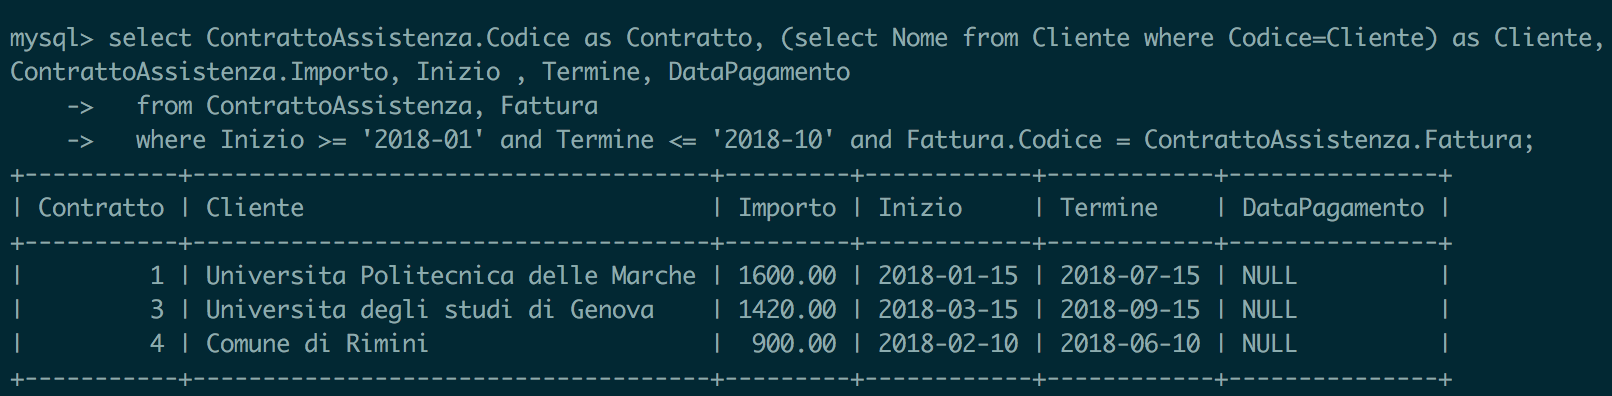
\includegraphics[width=\linewidth]{./immagini/op1}}
\newline\newline

\noindent\textit{Consultazione dati di una gara pubblica (in media cinque volte al giorno)}
\begin{verbatim}
select * from Gara where RichiestaMEPA = <numero_richiestamepa>;
\end{verbatim}
\vspace{1cm}

\noindent\textit{Consultazione dati di una trattativa diretta (in media due volte al giorno)}
\begin{verbatim}
select * from Trattativa where RichiestaMEPA = <numero_richiestamepa>;
\end{verbatim}
\vspace{1cm}

\noindent\textit{Consultazione caratteristiche di un prodotto (cinque volte al giorno)}
\begin{verbatim}
/* monitor per codice */
select Prodotto.Codice, Produttore, Modello, Dimensione, Risoluzione
  from Prodotto, Monitor
  where Prodotto.Codice = Monitor.Codice
  and Monitor.Codice = <codice_monitor>;

/* notebook per codice */
select Prodotto.Codice, Produttore, Modello, Processore, RAM, Storage,
  Schermo, SistemaOperativo
  from Prodotto, Notebook
  where Prodotto.Codice = Notebook.Codice
  and Notebook.Codice = <codice_notebook>;

/* pcdesktop per codice */
select Prodotto.Codice, Produttore, Modello, Processore, RAM, Storage,
  SistemaOperativo
  from Prodotto, PCDesktop
  where Prodotto.Codice = PCDesktop.Codice
  and PCDesktop.Codice = <codice_pcdesktop>;
\end{verbatim}
\vspace{0.5cm}

\noindent\makebox[\textwidth]{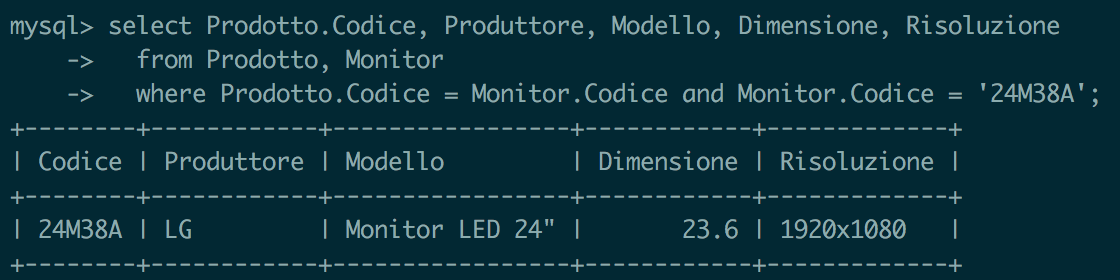
\includegraphics[width=\linewidth]{./immagini/op2}}
\newline\newline

\noindent\textit{Consultazione prezzo di un prodotto (dieci volte al giorno)}
\begin{verbatim}
select min(Prezzo) as Prezzo, Fornitore
  from Catalogo
  where Prodotto = <codice_prodotto> and InizioValidita < NOW()
  and FineValidita > NOW()
  group by Fornitore;
\end{verbatim}
\vspace{0.5cm}

\noindent\makebox[\textwidth]{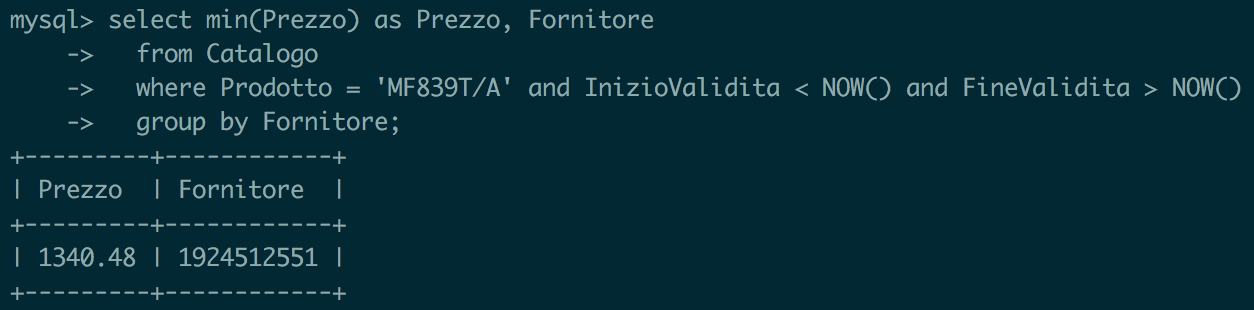
\includegraphics[width=\linewidth]{./immagini/op3}}
\newline\newline

\noindent\textit{Consultazione di una fattura (una volta al giorno)}
\begin{verbatim}
select * from Fattura where Codice = <codice_fattura>;
\end{verbatim}
\vspace{1cm}

\noindent\textit{Statistica delle gare pubbliche vinte e perse in un determinato periodo (una volta al mese)}
\begin{verbatim}
select Gara.RichiestaMEPA, Aggiudicatario, OffertaVincitore, LimiteSpesa
  from Gara, RichiestaMEPA
  where TermineOfferte >= <inizio_periodo>
  and TermineOfferte <= <fine_periodo>
  and Gara.RichiestaMEPA = RichiestaMEPA.Numero
  order by Aggiudicatario = 'Rimini Service' desc;
\end{verbatim}
\vspace{0.5cm}

\noindent\makebox[\textwidth]{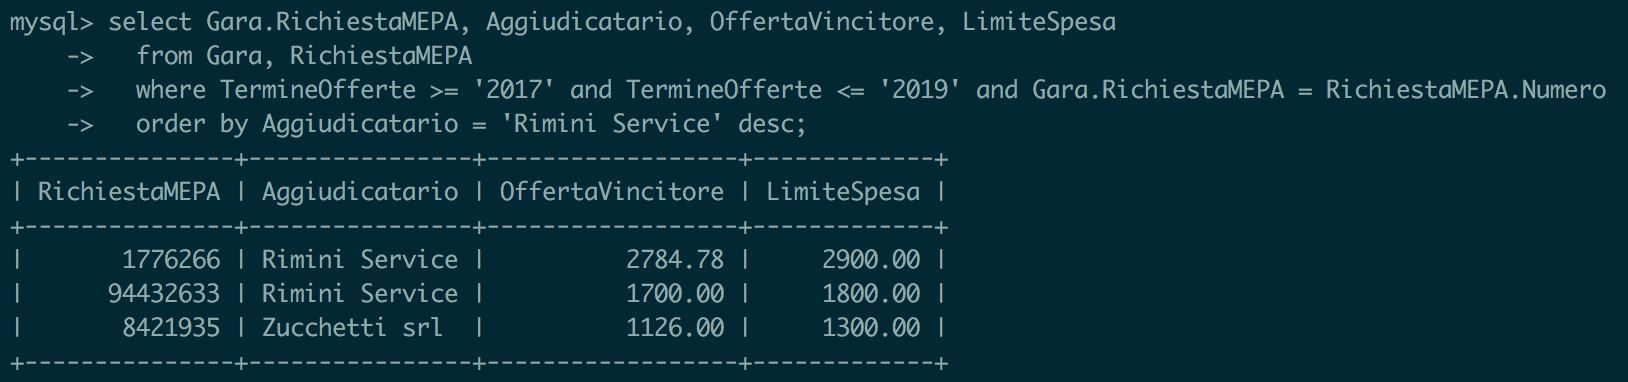
\includegraphics[width=\linewidth]{./immagini/op4}}
\newline\newline

\noindent\textit{Statistica delle trattative dirette stipulate (una volta al mese)}
\begin{verbatim}
select * from Trattativa order by Stipulata = true desc;
\end{verbatim}
\vspace{0.5cm}

\noindent\makebox[\textwidth]{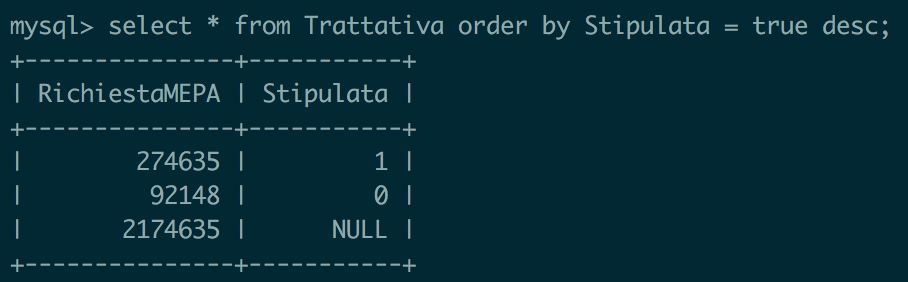
\includegraphics[width=\linewidth]{./immagini/op5}}
\newline\newline

\noindent\textit{Statistica dei prodotti più venduti (una volta al mese)}
\begin{verbatim}
select Codice, Quantita, Produttore, Modello
  from Vendita, Prodotto
  where Vendita.ProdottoServizio = Codice
  order by Quantita desc;
\end{verbatim}
\vspace{0.5cm}

\noindent\makebox[\textwidth]{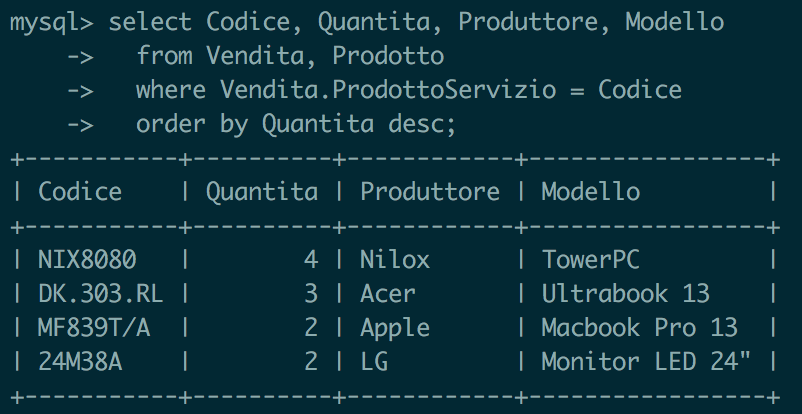
\includegraphics[width=0.7\linewidth]{./immagini/op6}}
\newline\newline

\noindent\textit{Statistica dei servizi più erogati (una volta al mese)}
\begin{verbatim}
select Servizio, count(*) as Frequenza
  from ElencazioneAssistenza
  group by Servizio
  order by Frequenza desc;
\end{verbatim}
\vspace{0.5cm}

\noindent\makebox[\textwidth]{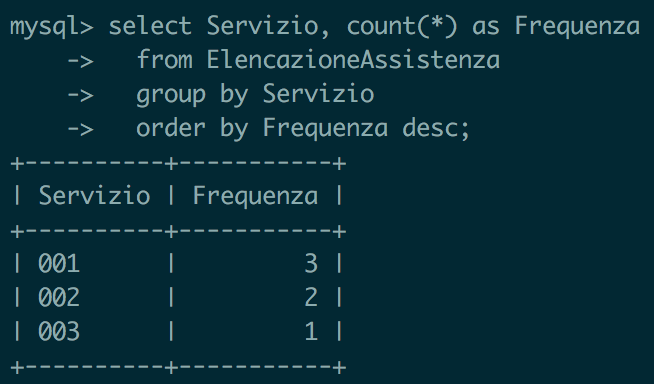
\includegraphics[width=0.6\linewidth]{./immagini/op7}}
\newline\newline

\noindent\textit{Verifica del pagamento delle fatture da parte dei clienti (due volte a settimana)}
\begin{verbatim}
select Codice, (select Nome from Cliente where Codice=Destinatario)
  as Nome, Emissione, Scadenza
  from Fattura
  where Emittente='Rimini Service' and NOW() >= Emissione
  and DataPagamento IS NULL
  order by Emissione;
\end{verbatim}
\vspace{0.5cm}

\noindent\makebox[\textwidth]{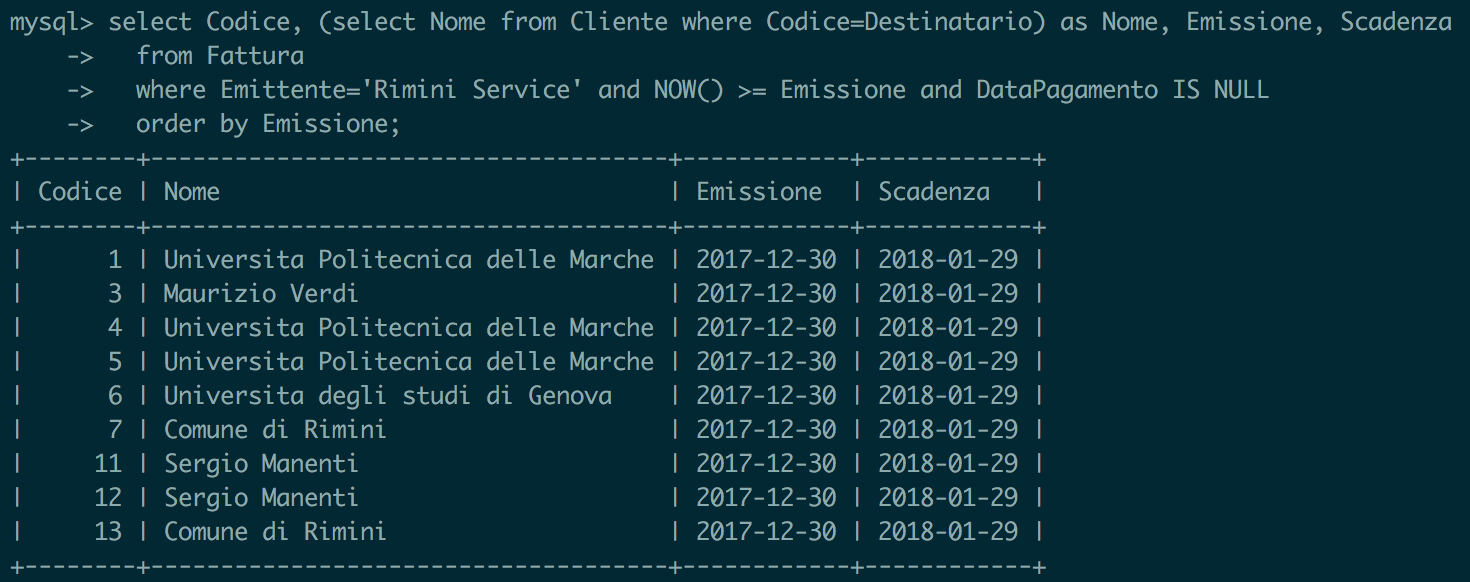
\includegraphics[width=\linewidth]{./immagini/op8}}
\newline\newline

\noindent\textit{Verifica di scadenza imminente del pagamento delle fatture da parte dei clienti (tre volte al mese)}
\begin{verbatim}
select Codice, (select Nome from Cliente where Codice=Destinatario)
  as Nome, Emissione, Scadenza
  from Fattura
  where Emittente='Rimini Service' and NOW() >= Emissione
  and DataPagamento IS NULL and DATEDIFF(Scadenza, NOW()) < 3
  order by Emissione;
\end{verbatim}
\vspace{0.5cm}

\noindent\makebox[\textwidth]{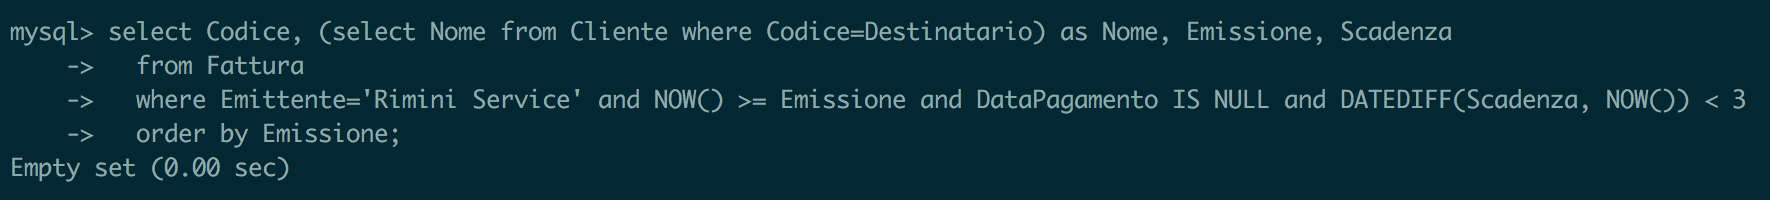
\includegraphics[width=\linewidth]{./immagini/op9}}
\newline\newline

\noindent\textit{Verifica del pagamento delle fatture da parte dell'azienda (due volte a settimana)}
\begin{verbatim}
select Codice, (select Nome from Fornitore where Codice=Emittente)
  as Fornitore, Emissione, Scadenza
  from Fattura
  where Destinatario='Rimini Service'
  and NOW() >= Emissione and DataPagamento IS NULL
  order by Emissione;
\end{verbatim}
\vspace{0.5cm}

\noindent\makebox[\textwidth]{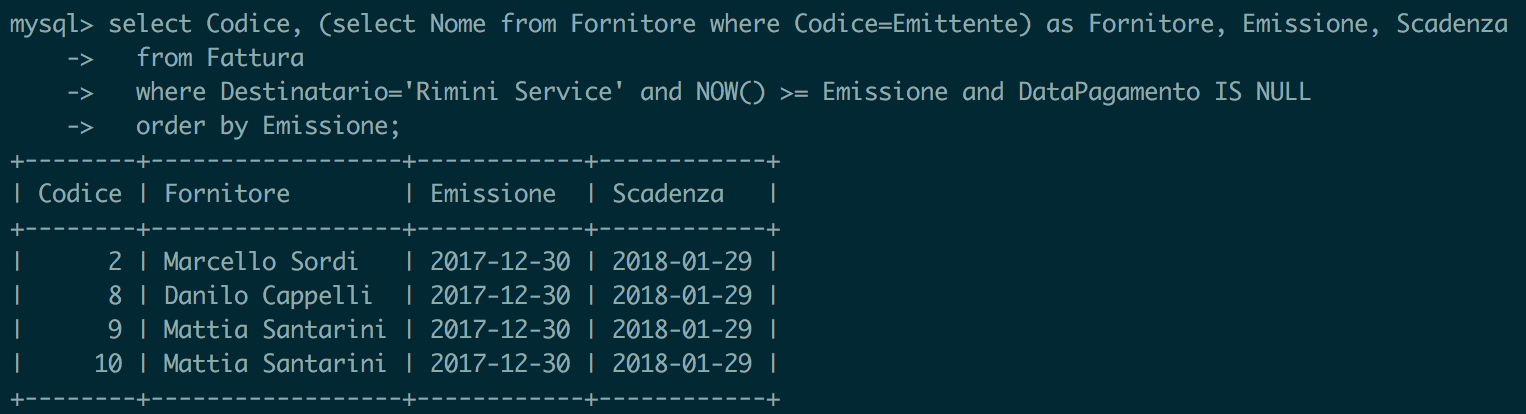
\includegraphics[width=\linewidth]{./immagini/op10}}
\newline\newline

\noindent\textit{Verifica di scadenza imminente del pagamento delle fatture da parte dell'azienda (tre volte al mese)}
\begin{verbatim}
select Codice, (select Nome from Fornitore where Codice=Emittente)
  as Fornitore, Emissione, Scadenza
  from Fattura
  where Destinatario='Rimini Service'
  and NOW() >= Emissione and DataPagamento IS NULL
  and DATEDIFF(Scadenza, NOW()) < 3
  order by Emissione;
\end{verbatim}
\vspace{0.5cm}

\noindent\makebox[\textwidth]{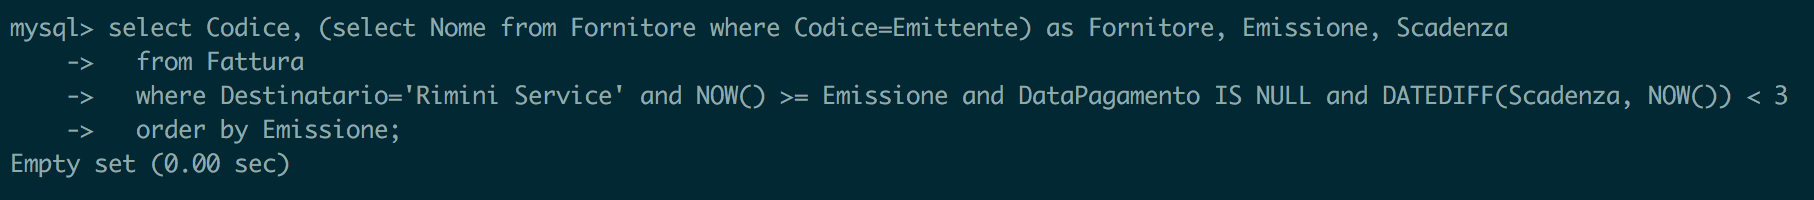
\includegraphics[width=\linewidth]{./immagini/op11}}
\newline\newline

\noindent\textit{Calcolo del guadagno netto ad una certa data (una volta al mese)}
\begin{verbatim}
select ((select sum(Importo) from Fattura where Emittente = 'Rimini Service')
  - (select sum(Importo) from Fattura where Emittente != 'Rimini Service'))
  as Guadagno;
\end{verbatim}
\vspace{0.5cm}

\noindent\makebox[\textwidth]{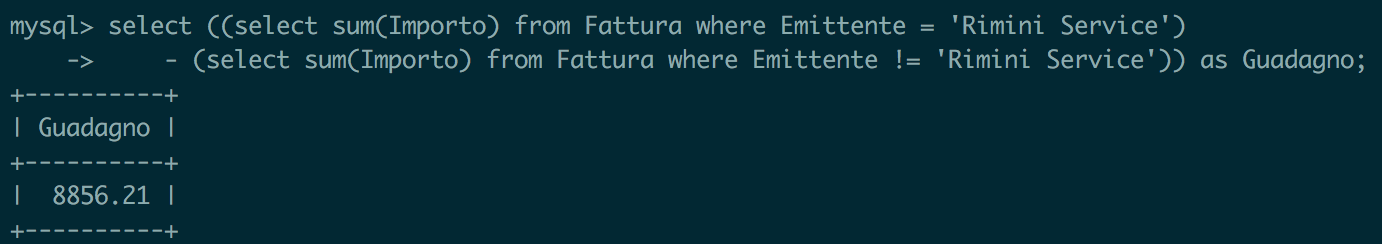
\includegraphics[width=\linewidth]{./immagini/op12}}
\newline\newline

\noindent\textit{Calcolo del volume di vendite in un determinato periodo (una volta al mese)}
\begin{verbatim}
select sum(Importo) as Volume_vendite
  from Fattura
  where Emittente = 'Rimini Service' and Emissione >= <inizio_periodo>
  and Emissione <= <fine_periodo>;
\end{verbatim}
\vspace{0.5cm}

\noindent\makebox[\textwidth]{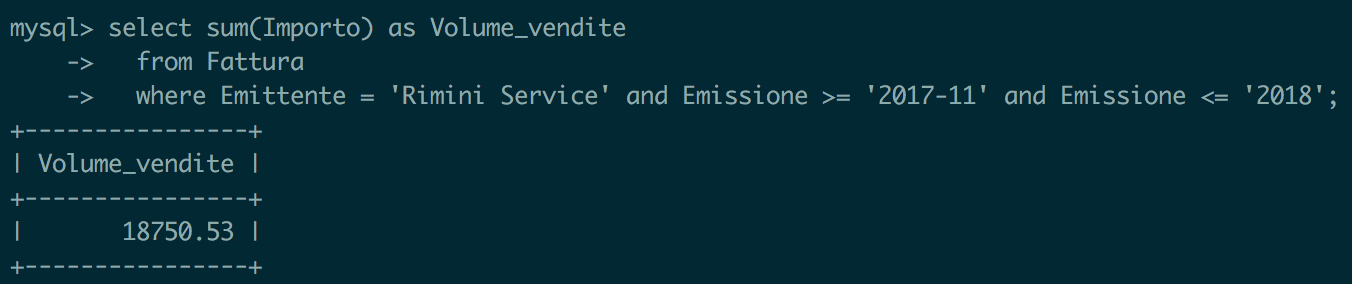
\includegraphics[width=\linewidth]{./immagini/op13}}
\newline\newline

\noindent\textit{Calcolo dei costi di spedizione di un'acquisto (tre volte al giorno)}
\begin{verbatim}
set @rank1:=0;
set @rank2:=0;
set @rank3:=0;
select Costo
  from CostoSpedizione
  where (select sum(Peso)
      from Prodotto
      where Codice IN (<lista_codici_prodotto>)) <= PesoMax
  and (select sum(Dim) from
    (select sum(Dim) as Dim from
    (
      (select @rank1:=@rank1+1 AS rank,
      SUBSTRING_INDEX(Dimensioni, 'x', 1) as Dim
      from Prodotto where Codice IN (<lista_codici_prodotto>))
    union all
      (select @rank2:=@rank2+1 AS rank,
      SUBSTRING_INDEX(SUBSTRING_INDEX(Dimensioni, 'x', 2), 'x', -1) as Dim
      from Prodotto where Codice IN (<lista_codici_prodotto>))
    union all
      (select @rank3:=@rank3+1 AS rank,
      SUBSTRING_INDEX(Dimensioni, 'x', -1) as Dim
      from Prodotto where Codice IN (<lista_codici_prodotto>))
    ) t
    group by rank) t) <= SommaMisureMax
  order by Costo limit 1;
\end{verbatim}
\vspace{0.5cm}

\noindent\makebox[\textwidth]{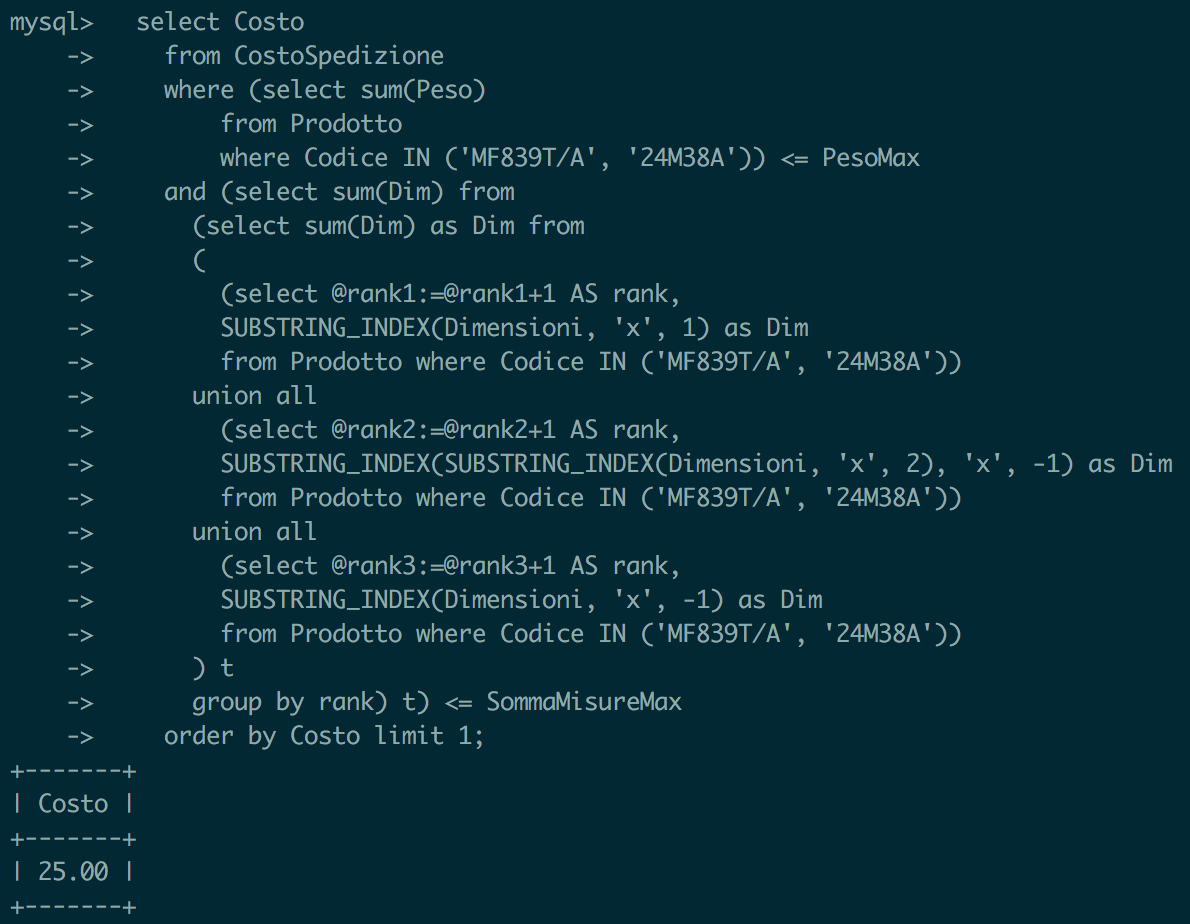
\includegraphics[width=0.85\linewidth]{./immagini/op14}}
\newline\newline

\noindent\textit{Selezione della migliore combinazione di prodotti (tre volte al giorno)}
\begin{verbatim}
select min(Prezzo) as Prezzo, Prodotto,
  (select Nome from Fornitore where Codice=Fornitore) as Fornitore
  from Catalogo
  where Prodotto IN <lista_codici_prodotto>
  and InizioValidita < NOW() and FineValidita > NOW()
  group by Prodotto;
\end{verbatim}
\vspace{0.5cm}

\noindent\makebox[\textwidth]{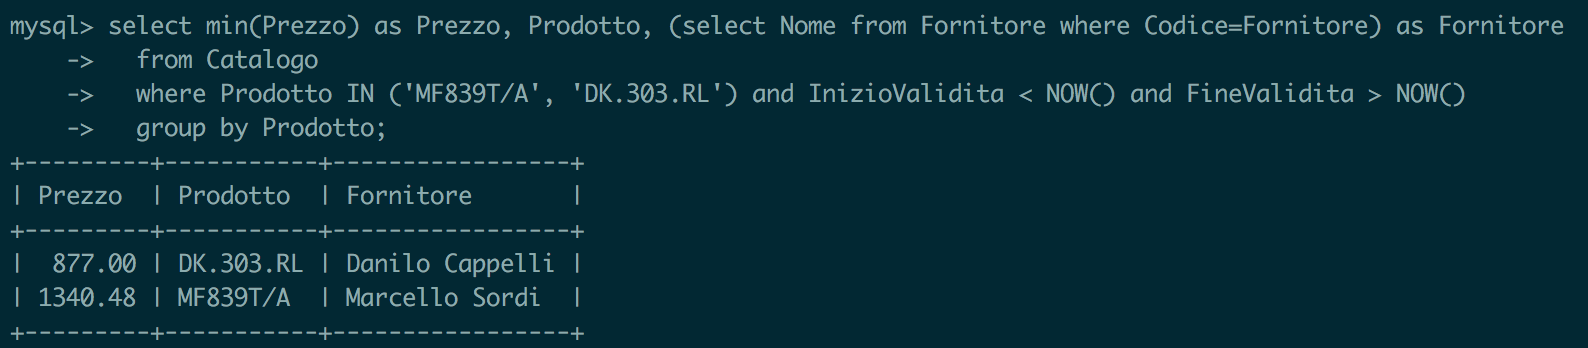
\includegraphics[width=\linewidth]{./immagini/op15}}
\newline\newline
